\section{A Real Time Spectrum Analyser Using LMS}
\subsection{LS solution and relationship to DFT}
Given the cost function $\mathcal{J}(\mathbf w)$between estimated signal $\mathbf {\hat y}(n)=\mathbf{F}\mathbf{w}$ and true signal $\mathbf y(n)$,
\begin{align}
\min_{\mathbf{w}}\|\mathbf{y}-\mathbf {\hat y}\|^2
&=\min_{\mathbf{w}}\|\mathbf{y}-\mathbf {\hat y}\|^H \|\mathbf{y}-\mathbf {\hat y}\|\notag\\
&=\min_{\mathbf{w}}(\mathbf{y}-\mathbf{F}\mathbf{w})^H (\mathbf{y}-\mathbf{F}\mathbf{w}) \notag\\
&=\min_{\mathbf{w}}(\mathbf{y}^H\mathbf{y}-\mathbf{y}^H\mathbf{F}\mathbf{w}-\mathbf{w}^H\mathbf{F}^H\mathbf{y}+\mathbf{w}^H\mathbf{F}^H\mathbf{F}\mathbf{w})
\label{eq:cost}
\end{align}
Thus, in order to minise the cost function, take the derivation with respect to $\mathbf w$ and equal to zero. The optimal weight can be obtained.
\begin{align}
\frac{\partial \mathcal{J}}{\partial \mathbf{w}} 
&=-\mathbf{F}^H\mathbf{y}-\mathbf{F}^H\mathbf{y}+2\mathbf{F}^H\mathbf{F}\mathbf{w}=0\notag\\
\mathbf{w}&=(\mathbf{F}^H\mathbf{F})^{-1}\mathbf{F}^H\mathbf{y}
\label{eq:ls}
\end{align}
The DFT of a sequence $x(n)$ is defined as
\begin{align}
X_k =\sum_{n=0}^{N-1}\hat x_n e^{-j2\pi kn/N}=\sum_{n=0}^{N-1}\hat x_n W^{nk}_N
\label{eq:dft}
\end{align}
where $W_N=e^{-j2\pi/N}$. In vector expression of Eq.\ref{eq:dft}, it is 
\begin{align}
\mathbf{X=W\hat x}
\end{align}
where transformation matrix $\mathbf{W} is$
\begin{align}
\mathbf{W}=
\begin{bmatrix}
    1 & 1 & 1 & \dots  & 1 \\
    1 & W_N & W_N^2 & \dots  & W_N^{N-1} \\
    \vdots & \vdots & \vdots & \ddots & \vdots \\
    1 & W_N^{N-1} & W_N^{2(N-1)} & \dots  & W_N^{(N-1)^2}
\end{bmatrix}
\end{align}
Due to the transformation matrix $\mathbf{W}$ is orthogonal and symmetric, the DFT is unitray transform. Therefore, the IDFT is 
\begin{align}
\mathbf{\hat x=W^{-1}X}\quad \text{with}\quad \mathbf{W^{-1}}=\frac{1}{N}\mathbf{W^H}
\end{align}
Which is corresponding to the estimated signal $\mathbf {\hat y}=\mathbf{F}\mathbf{w}$. Thus, the Eq.\ref{eq:ls} can be expressed as
\begin{align}
\mathbf{w}
=(\mathbf{F}^H\mathbf{F})^{-1}\mathbf{F}^H\mathbf{y}
=(N\mathbf{F^{-1}F})^{-1}\mathbf{F}^H\mathbf{y}
=N\mathbf{F}^H\mathbf{y}
=\mathbf F^{-1}\mathbf{y}
\end{align}
where is corresponding to the DFT $\mathbf{X=W\hat x}$.
\subsection{Projection and baiss of DFT}
Due to the transformation matrix of DFT is symmetric and orthogonal, the Fourier trainsfrom coefficients $\mathbf{w}$ is formed by projecting the signal $y(n)$ onto the transformation matrix $\mathbf{W}$ which is composed of harmonical sinusoids basises. In contrast, the IDFT is the inversely process to reconstruct the original signal by superposition of sinusoidal projections. However, the DFT and IDFT use finite length $N$ to estimate either coefficients $\mathbf{w}$ or signal $\mathbf{\hat y}$, which makes errors occur comparing with true value.
\subsection{DFT-CLMS}
The DFT-CLMS algorithm is implimented on the non-stationary FM signal. Fig.\ref{fig:3_3_c1} depicts the estimated time-varying frequencies. The trend of frequency is generally captured especially in perfectly estimation for constant segment. However, there exists an issue that the estimated frequency remains till the end of time index once it was obtained. Thus, the weights are not updated, which presents long smears in spectrum. The reason which causes this problem is that the gradient of back-propagation vanishes. Due to the gradient of the LMS algorithm is based on the eigenvalues of autocorrelation matrix. For the harmonically related sinusoids $\mathbf x(n)$, there are zero eigenvalues of $\mathbf R_{xx}$, resulting in hard back-propagation. 
\begin{figure}[htb]
     \centering
     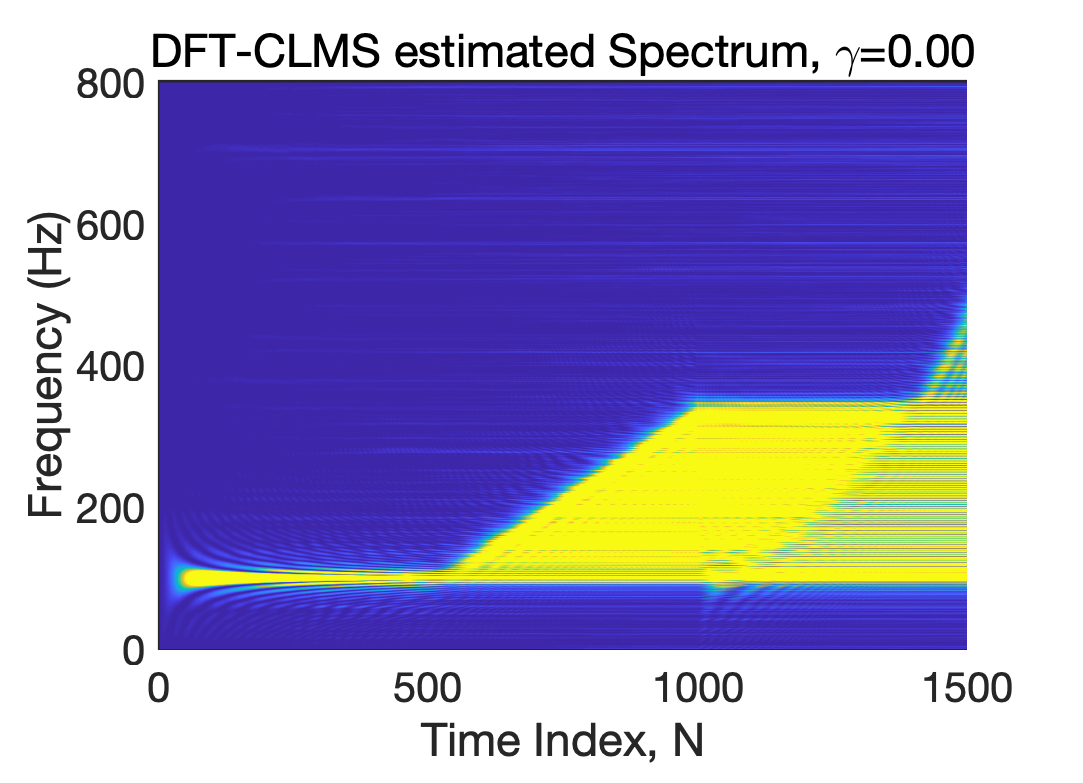
\includegraphics[width=0.4\textwidth]{fig/33/33c1.eps}
     \caption{DFT-CLMS: estimated FM frequency}
     \label{fig:3_3_c1}
\end{figure}\\
To solve this problem, the Leaky CLMS is applied on the weight update with leakage coefficient, in expression of $\gamma$ $\mathbf{w}(n+1)=(1-\gamma\mu)\mathbf{w}(n)+\mu e^*(n)\mathbf x(n)$. By changing previous value of weight, the weight will update along time. Fig.\ref{fig:3_3_c2} illustrated the performance affected by different $\gamma$. With small value of $\gamma$, most of smears are removed presented as relatively distinct trends. The optimal value of $\gamma$ is 0.1 with acceptable bias. If the leakage coefficient is too large, the estimation is inaccurate due to the large bias added.
\begin{figure}[htb]
     \centering
     \hspace{-0.4cm}
     \begin{subfigure}[b]{0.33\textwidth}
         \centering
         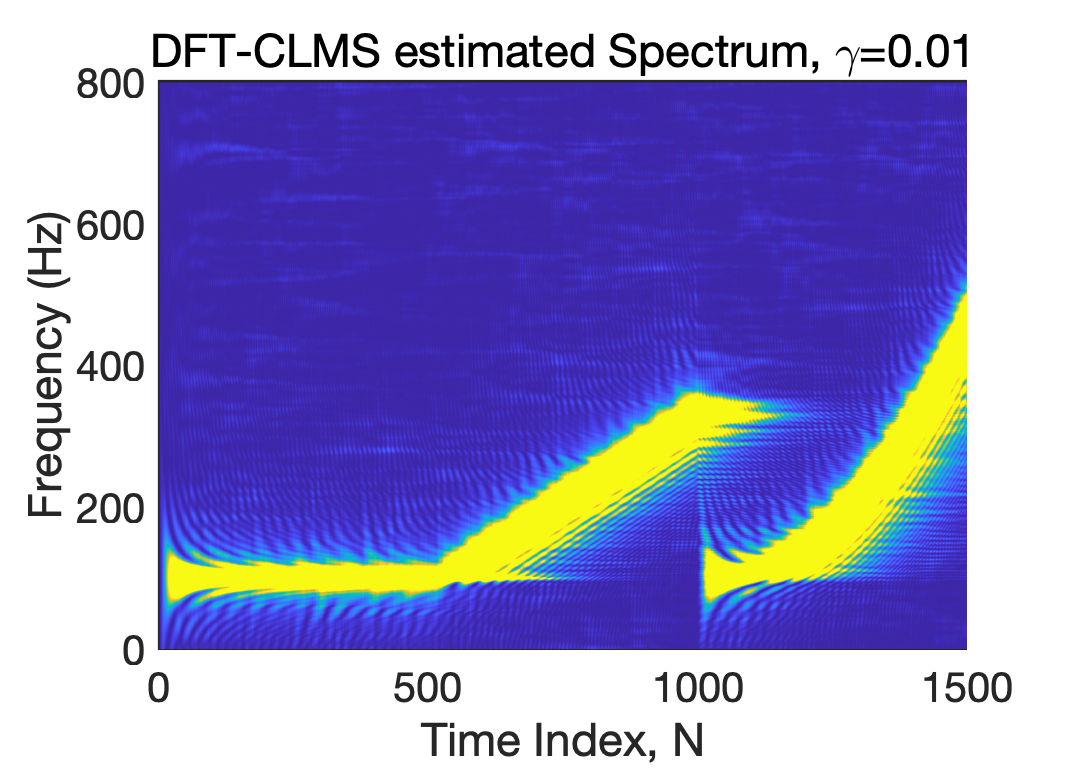
\includegraphics[width=\textwidth]{fig/33/33c2.eps}
     \end{subfigure}
    \hspace{-0.4cm}
     \begin{subfigure}[b]{0.33\textwidth}
         \centering
         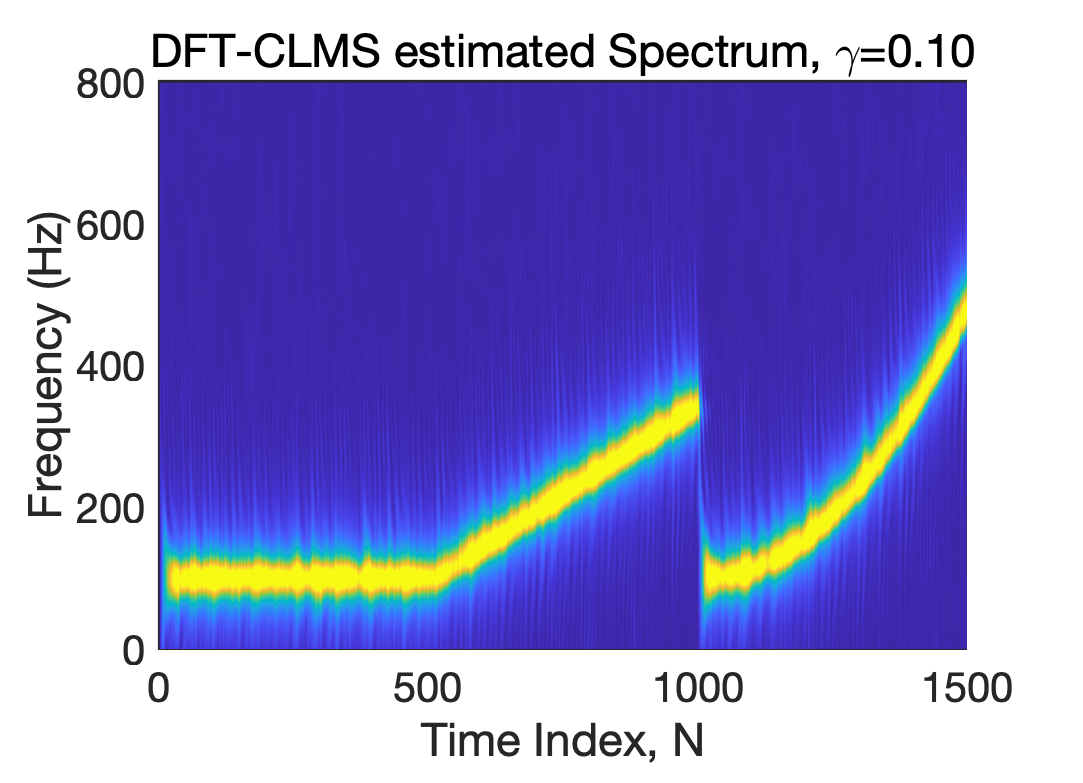
\includegraphics[width=\textwidth]{fig/33/33c3.eps}
     \end{subfigure}
    \hspace{-0.4cm}
     \begin{subfigure}[b]{0.33\textwidth}
         \centering
         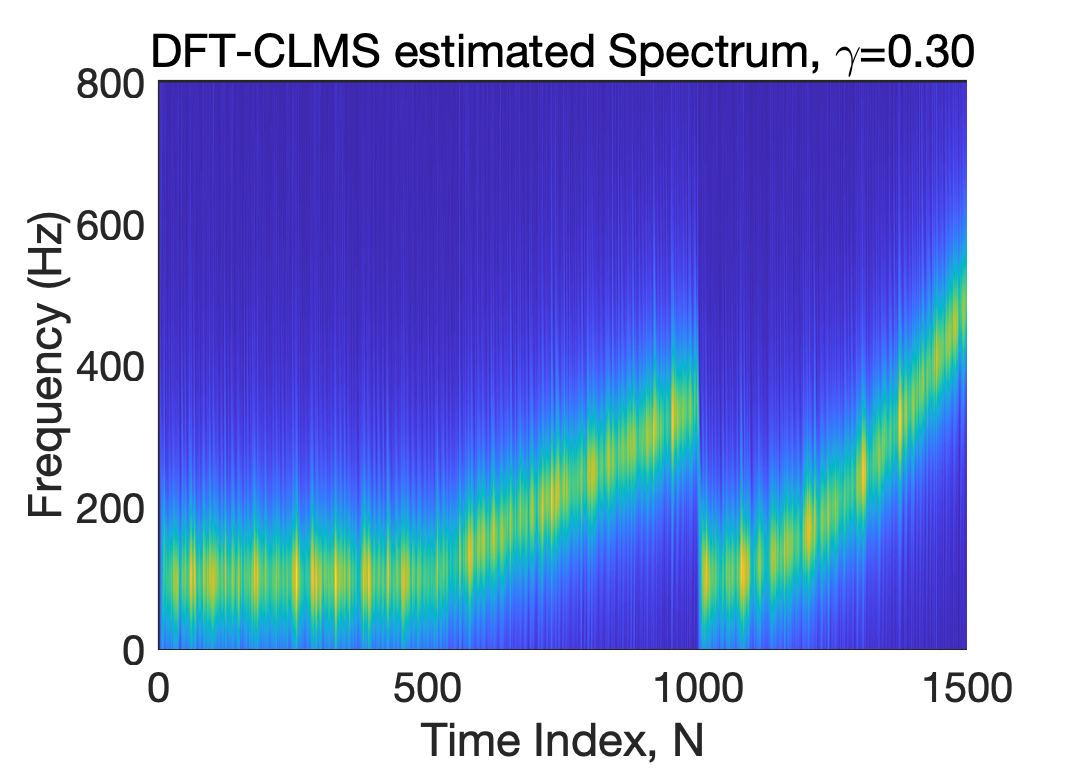
\includegraphics[width=\textwidth]{fig/33/33c4.eps}
     \end{subfigure}
     \hspace{0.4cm}
        \caption{Leaky DFT-CLMS: estimated FM frequency with different $\gamma$}
        \label{fig:3_3_c2}
\end{figure}
\subsection{DFT-CLMS estimated EEG signal}
The DFT-CLMS algorithm can also be used to analyse EEG signal. As shown in Fig.\ref{fig:3_3_d}, the estimated spectrum agrees with the analysis in Part 1.2(b). A strong response at 8-10$Hz$ called alpha-rhythm is clear shown. The SSVEP at 13$Hz$ is detected as well, following its harmonic frequency at $26Hz$. However, the harmonic frequency at $39Hz$ is hard to recognize. Moreover, the recording apparatus is strongly detected at $50Hz$.\\
Nevertheless, the Leaky CLMS algorithm is not suitable for EEG data, since the EEG \texttt{POz} is stationary signal. Thus, adding a leakage coefficient results in adding bias on the correct estimations.
\begin{figure}[htb]
     \centering
     \hspace{0.4cm}
     \begin{subfigure}[b]{0.4\textwidth}
         \centering
         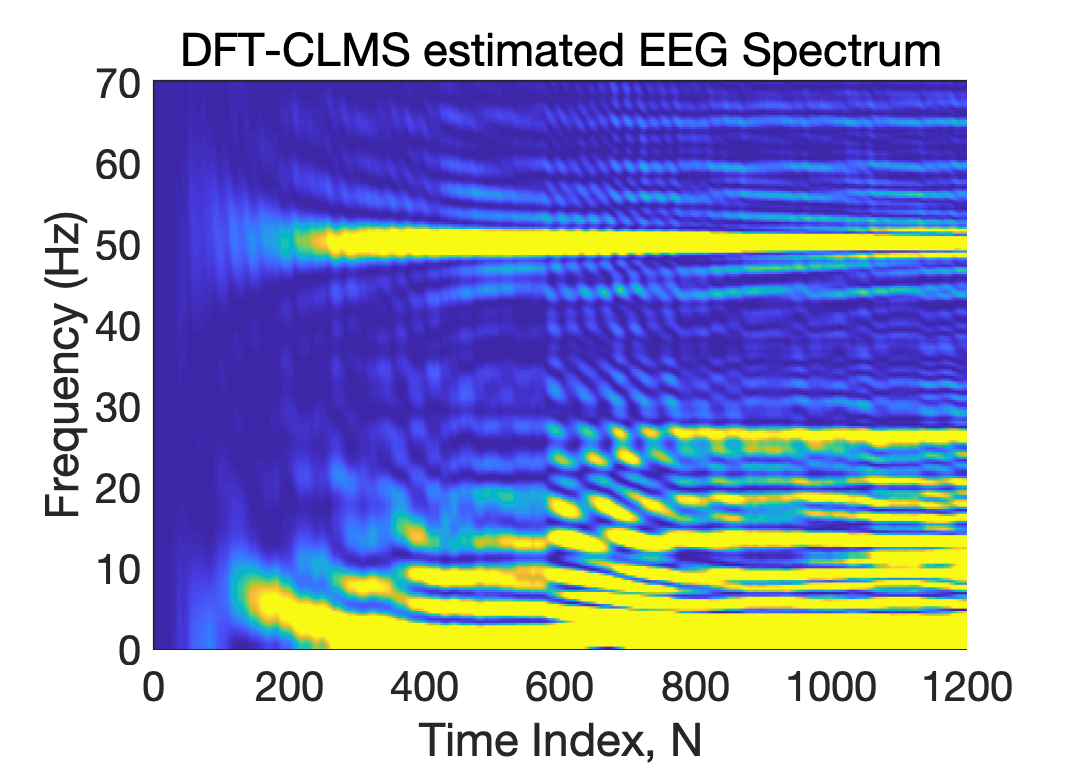
\includegraphics[width=\textwidth]{fig/33/33d1.eps}
     \end{subfigure}
    \hspace{0.4cm}
     \begin{subfigure}[b]{0.4\textwidth}
         \centering
         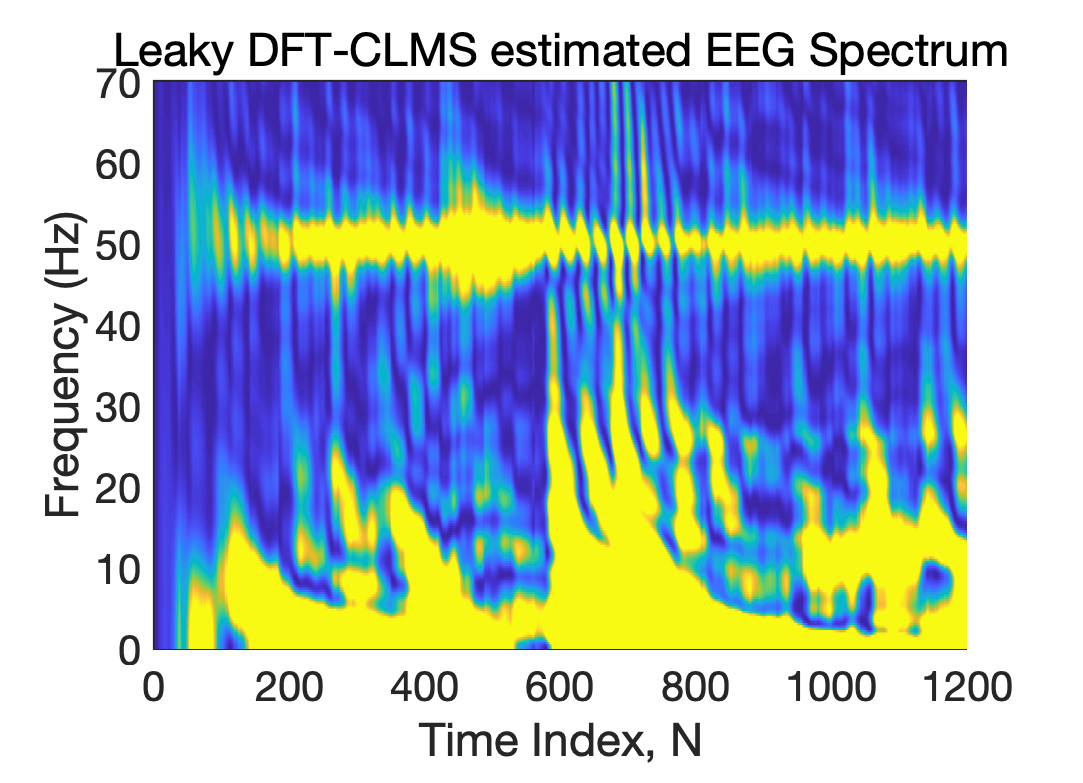
\includegraphics[width=\textwidth]{fig/33/33d2.eps}
     \end{subfigure}
     \caption{DFT-CLMS: estimated EEG frequency}
     \label{fig:3_3_d}
\end{figure}